\section{Sesión 1 - 5 de julio de 2021}

\begin{nota}
	La teoría a continuación se refiere a funciones acotadas.
\end{nota}

\begin{definicion}
	Una \textbf{partición} $P$ del intervalo $[a,b]$ es un conjunto finito: $P=\{x_0,x_1,x_2,\cdots, x_n\}$ donde $a=x_0<x_1<\cdots < x_n=b$. 
\end{definicion}

\begin{nota}
	$P[a,b]$ denota el conjunto de todas las particiones de $[a,b]$. 
\end{nota}

\begin{nota}
	\begin{enumerate}
		\item Una partición $P'\in P[a,b]$ es un \textbf{refinamiento} de $P\in P[a,b]$, si $P\subset P'$ 
		\begin{center}
			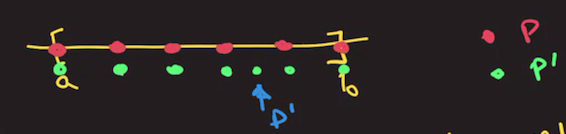
\includegraphics[scale=0.5]{images/1/1}
		\end{center}
	\textbf{Notación:} si $P\subset P'\implies$ Se denota: $P'\preceq P$. 
	\begin{enumerate}
		\item $P\preceq P (\iff P\subset P), \ \forall P\in P[a,b]$. 
		\item Si $P'\preceq P$ y $P\preceq P'\implies P=P'$. 
		\item Si $P'\preceq P$ y $P''\preceq P'\implies P''\preceq P$. 
	\end{enumerate}
$\implies$ La relación $\preceq$ es de orden parcial. 
\item Para $P\in P[a,b], \Delta x_k:=x_k-x_{k-1}$, es la longitud del $k$-ésimo subintervalo en la partición. Nótese que: 
$$\sum_{k=1}^{n}\Delta x_k=b-a$$
\item La norma o malla de $P\in P[a,b]$ se define:  $\lVert P \rVert =\max\{\Delta x_k:k=1,2,\cdots, n\}$. Note que, si $P'\preceq P\implies \lVert P'\rVert \preceq \lVert P\rVert$.
	\end{enumerate}
\end{nota} 

\begin{definicion}
	Sea $P\in P[a,b]$ y sean, para $k=1,\cdots, n$, 
	$$M_k(f)=\sup\{f(x): x\in [x_{k-1},x_k]\}$$
	$$m_k(f)=\inf\{f(x):x\in [x_{k-1},x_k]\}$$
	Entonces, los números: 
	$$U(P,f)=\sum_{k=1}^{n}M_k(f)\Delta x_k,\quad L(P,f)=\sum_{k=1}^{n}m_k(f)\Delta x_k$$
	se llaman la suma superior e inferior de Darboux de $f$ para partición $P$. 
		\begin{center}
		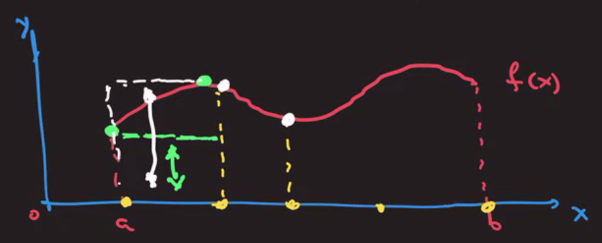
\includegraphics[scale=0.5]{images/1/2}
	\end{center}
\end{definicion}

\begin{prop}
	Sean $P,P',P_1,P_2\in P[a,b]$. Entonces, 
	\begin{enumerate}
		\item $$P'\preceq P\implies 
			P'\preceq P\implies \begin{cases}
				U(P',f)\leqslant U(P,f)\\
				L(P',f)\geqslant L(P,f)
		\end{cases}$$
	\item $$L(P_1,f)\leq U(P_2,f)$$
	\end{enumerate}
\end{prop}

\begin{proof}
	Tenemos: 
		\begin{center}
		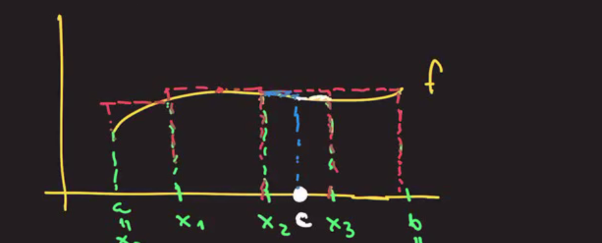
\includegraphics[scale=0.5]{images/1/3}
	\end{center}
	\begin{enumerate}
		\item Sea $P'=P\cup \{c\}$ y suponga que $c\in [x_{i-1},x_i]\subset P\implies U(P',f)=\sum_{\substack{k=1\\ k\neq i}}^{n}M_k(f)\Delta x_k+M'(c-x_{i-1})+M''(x_i-c)$. Como $M'\leq M_i(f)$ y $M''\leq M_i(f)$. $\implies U(P',f)\leq \sum_{\substack{k=1\\k\neq i}}^{n}M_k(f)\Delta x_k + M_i(f)\underbrace{[(c-x_{i-1})+(x_i-c)]}_{\Delta x_i}=\sum_{k=1}^{n} M_k(f)\Delta x_k=U(P,f)$. 
		\item Como $P_1,P_2\in P[a,b]$, sea $P=P_1\cup P_2$. Como $P\preceq P_1$ y $P\preceq P_2$, entonces $L(P_1,f)\leq L(P,f)\leq U(P,f)\leq U(P_2,f)$.
	\end{enumerate}
\end{proof}

\begin{definicion}
	\begin{enumerate}
		\item Se define la integral superior de Riemman de $f$ sobre $[a,b]$. 
	$$\overline{\int_a^b}f=\inf\{U(P,f):P\in P[a,b]\}$$
		\item Se define la integral interior de Riemman de $f$ sobre $[a,b]$. 
	$$\underline{\int_a^b}f=\sup\{L(P,f):P\in P[a,b]\}$$
	\end{enumerate}
\end{definicion}
\begin{ejemplo}
	Sea $f:[a,b]\to \mathbb{R}\ni f(x)=c$.
	\begin{enumerate}
		\item $ U(P,f)=\sum_{k=1}^{n}c\Delta x_k=c\sum_{k=1}^{n}\Delta x_k=c(b-a)\implies \overline{\int_a^b}f=\inf \{U(P,f):P\in P[a,b]\}=c(b-a)$.
		\item $ L(P,f)=\sum_{k=1}^{n}c\Delta x_k=c\sum_{k=1}^{n}\Delta x_k=c(b-a)\implies \underline{\int_a^b}f=\sup \{L(P,f):P\in P[a,b]\}=c(b-a)$
	\end{enumerate}
\end{ejemplo}

\begin{ejemplo}
	Sea $f:[0,1]\to\mathbb{R}\ni$
	$$f(x)=\begin{cases}
		1&, x\in\mathbb{Q}\\
		0&, x\in \mathbb{I}rr
	\end{cases}$$
Sea $P\in P[0,1]$. Entonces, 
\begin{enumerate}
	\item $U(P,f)=\sum_{k=1}^{n}1\Delta x_k=\sum_{k=1}^{n}\Delta x_k=1-0=1\implies \overline{\int_0^1}f=\inf\{\underbrace{U(P,f)}_1:P\in P[0,1]\}=1$.
	\item $L(P,f)=\sum_{k=1}^{n}0\Delta x_k=0\implies \underline{\int_0^1}f=\sup\{\underbrace{L(P,f)}_0:P\in P[0,1]\}=0$. 
\end{enumerate}
\end{ejemplo}
